% Updated Mapping
This section presents the results of the updated mapping and 
compares them with results from the 2013 SMS.

\begin{figure*}[t]
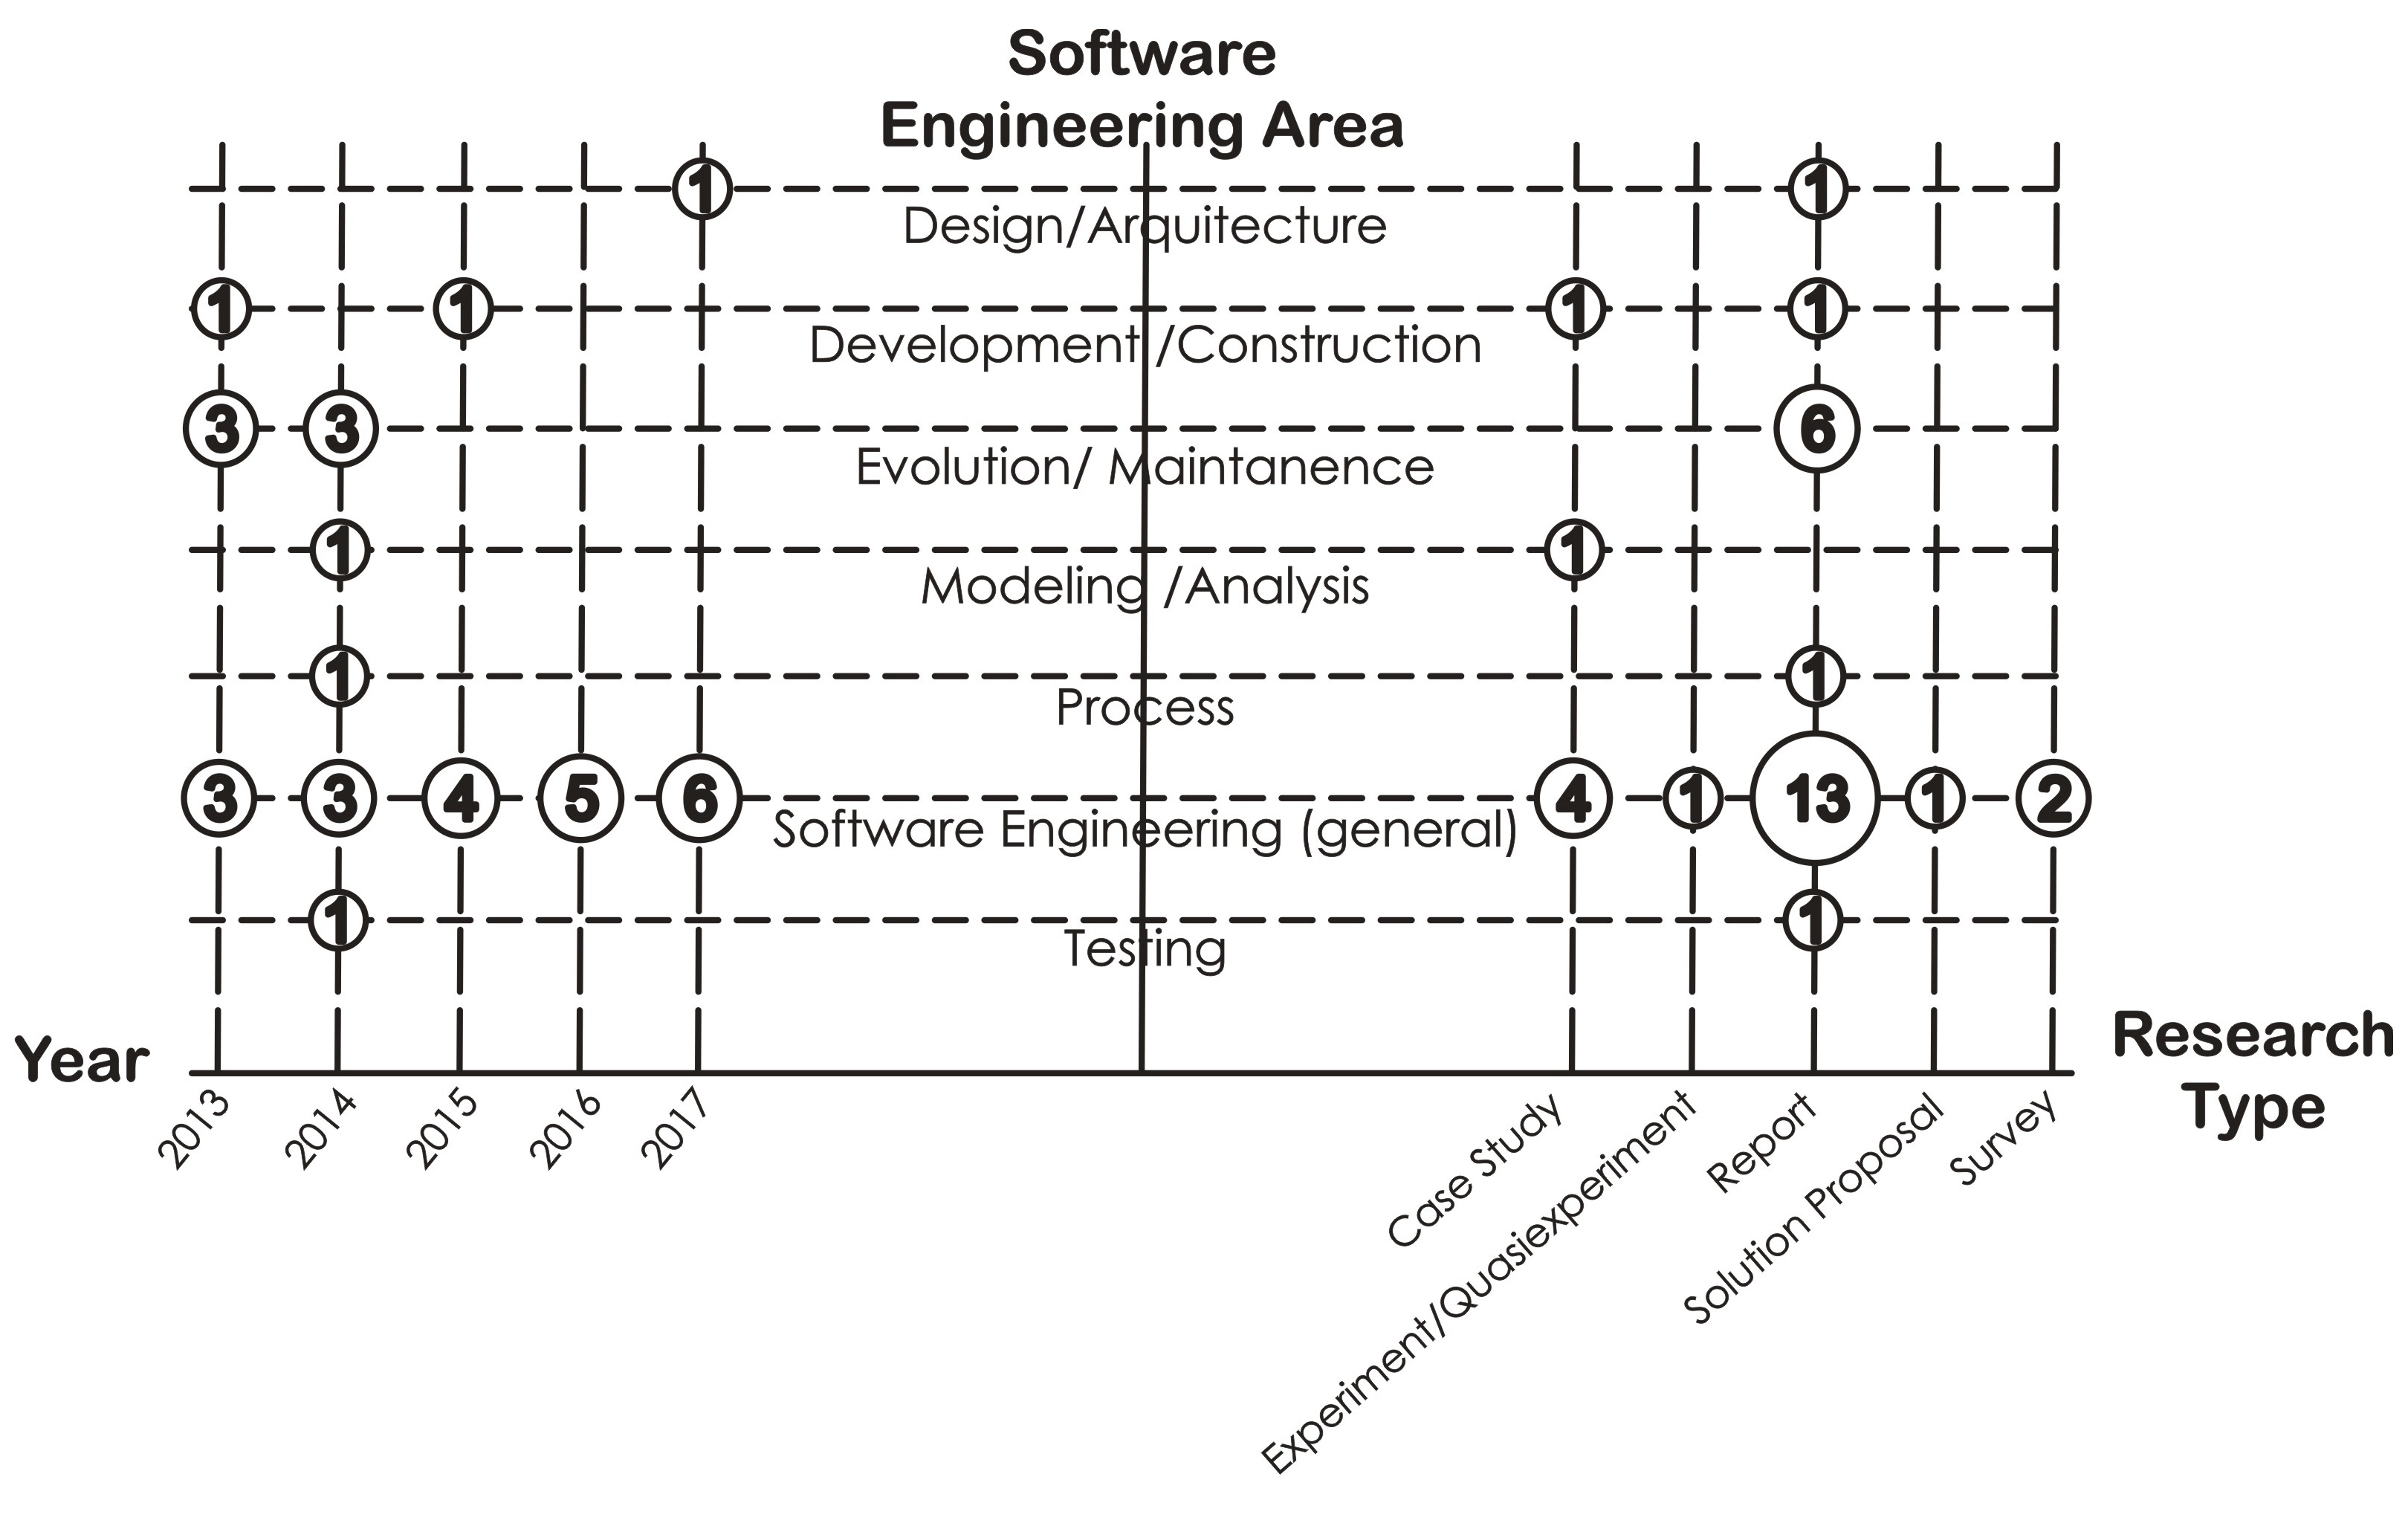
\includegraphics[width=0.8\linewidth]{fig/mapa01.jpg} 
\caption{Software engineering area vs. year vs. research type.} \label{fig:mapa01}
\end{figure*}

\subsection{Overview of study objectives and contributions}

We have identified several approaches in the selected papers. One of the main challenges of using FLOSS in SE education is selecting projects for use in a course. Some studies address the choice of suitable projects, providing a predefined list of FLOSS \cite{id0135, id5357, id5676}. \citeauthor{id0135} made available a list of seventeen projects compatible with students' background. The selected projects ranged in size from 5,500 to 10,500 lines of code. \citeauthor{id5357} have listed ten open source projects for exploring, experimenting and choice by students. In the study of \citeauthor{id5676}, students choose the project from a list presented in the classroom. 
%
In some studies, students freely choose the project they wanted to work during the course 
\cite{id1088, id17882}. 
In the study presented by \citeauthor{id1088}, teams were able to freely choose a project to carry out their practices and apply the software development techniques learned in lectures. 
\citeauthor{id17882} let students choose a software system to study its architecture and to document the system. 
In the study of \citeauthor{id0093}, authors specify a set of criteria to aid the selection process. Groups of up to six students undertook a search for projects hosted in the SourceForge, GitHub and GoogleCode repositories. \citeauthor{id1192} previously established that students should work with the JabRef project, an open source bibliographic reference manager.

Some studies present techniques for using FLOSS in SEE \cite{id0106, id0134, id1192, id17800, id5676}. \citeauthor{id0106} used the Wilcoxon Mann-Whitney test, a non-parametric statistical hypothesis test, to compare two related samples. The result of their tests led to reject the null hypothesis that confirmed the efficacy of the method. 
In their study, \citeauthor{id0134} subjected students 
to the technique of visualizing algorithms, showing parameters, relevant variables, 
and visual representation of manipulated objects, as well as a formal description of the algorithm. Students reported that software visualization tools are easy to use and help understand software structure, behavior, and complexity. 
\citeauthor{id1192} used gamification to guide and motivate students to contribute to FLOSS projects. \citeauthor{id17800} provided a tutorial to help instructors identify appropriate software projects, design the set of tasks for students, and select useful tools. \citeauthor{id5676} used a hybrid approach combining distance-based project learning, providing printed materials (e.g., books, tutorials and articles), online resources and classroom lectures.

We identified tools that served to support the use of open source projects in SEE \cite{id1088, id17882, id5357, id0089, id5676}. \citeauthor{id1088} and \citeauthor{id17882} used the Github version control system to maintain project code and track individual student contributions. In the study of \citeauthor{id5357}, student pairs were able to develop, test, and debug small Java programs using Eclipse and to create UML class diagrams. The study of \citeauthor{id0089} reports the experience of an open source software community using the GitLab teaching environment to support students' collaborative software development activities. \citeauthor{id5676} gave their students access to the FLOSSCom and OpenSE virtual learning environments.

Other studies have described their assessment processes \cite{id4663, id0093, id0089, id5676}. 
For \citeauthor{id4663}, project grade accounts for 70\% of students' scores. They considered product usefulness, maintenance capacity, extension of software design, verification effectiveness, teamwork and final presentation. In~\cite{id0093}, students were assessed from code presentation, participation in communication channels, documentation submitted at each stage, comments from peer review and contribution to the FLOSS community repository. To assess students, \citeauthor{id0089} considered push, pull, and commit records that students performed using GitLab. Finally, in \cite{id5676} the assessment considered the quality of produced work, documentation clarity and usefulness, number of bugs reported, complexity and effectiveness of developed code, and analysis depth and usefulness.

% Mapa02 aqui - burlando latex
\begin{figure*}[htb]
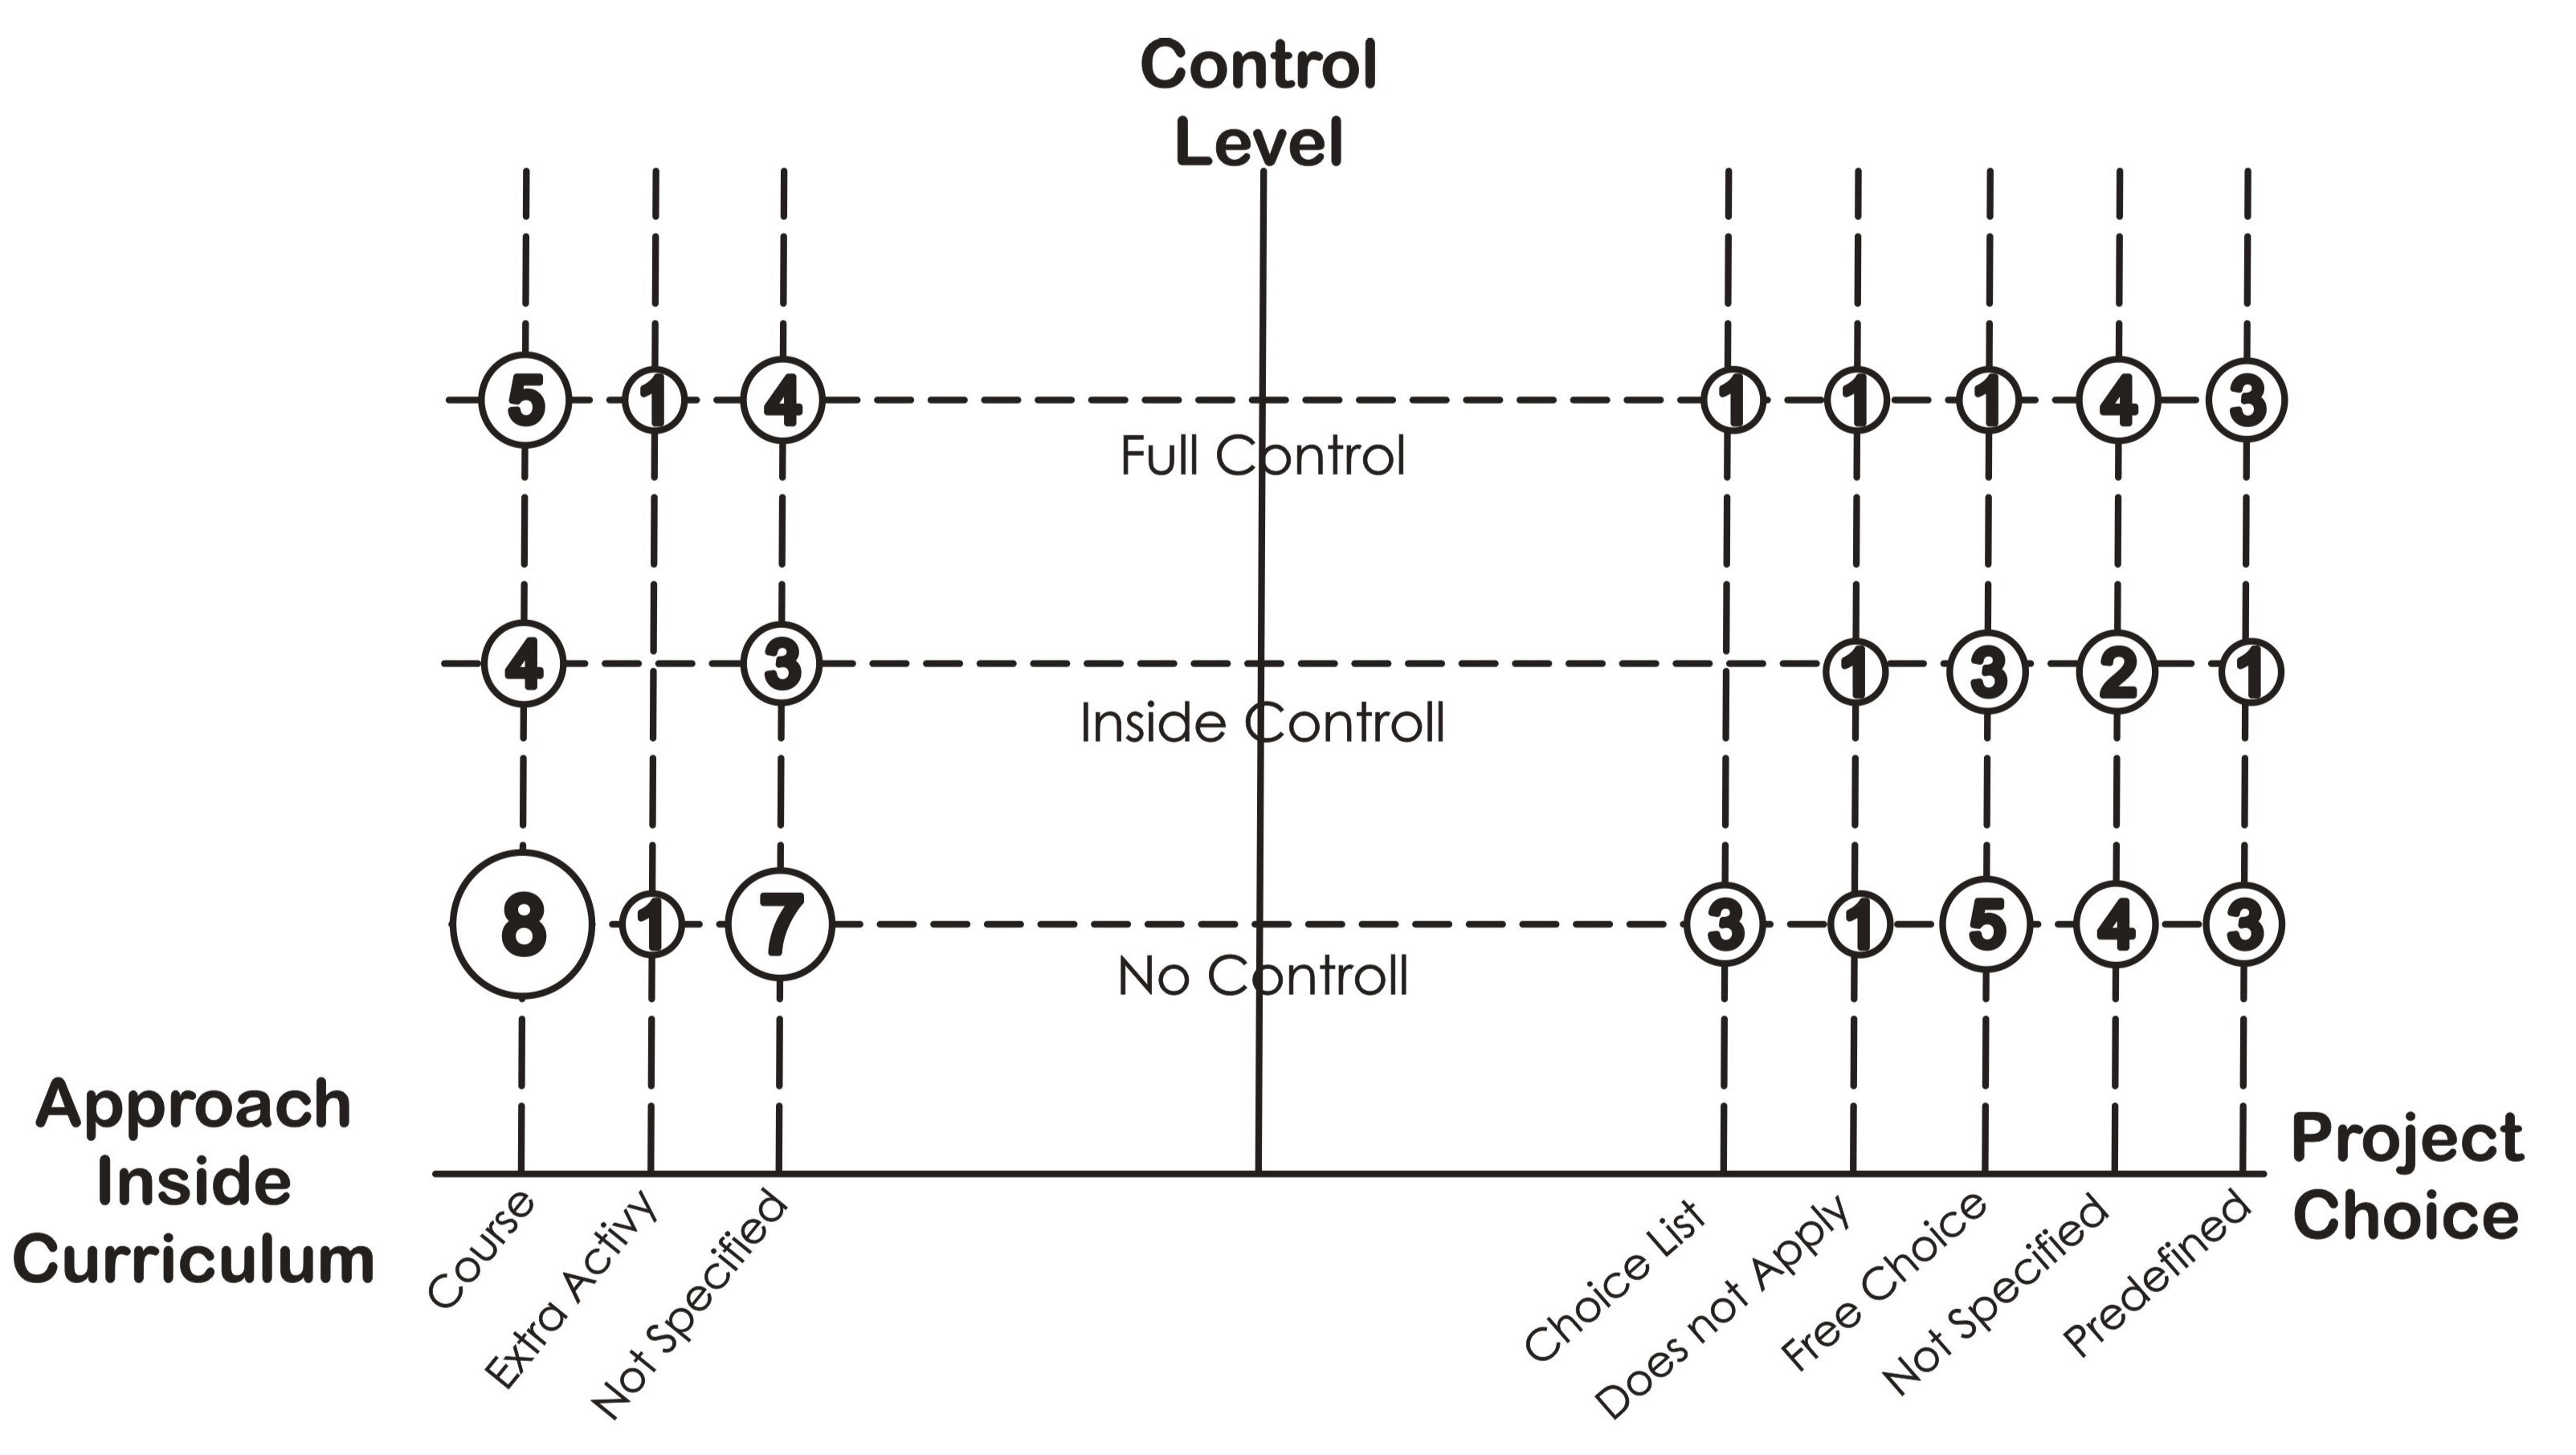
\includegraphics[width=0.7\linewidth]{fig/mapa02.jpg}
\caption{Curriculum choice vs. control level vs. project choice.} \label{fig:mapa03}
\end{figure*}

\subsection{FLOSS projects in SEE}

The main purpose of our SMS update was to discover 
how FLOSS projects have been used in SEE (RQ1) 
over the last five years. 
Figure~\ref{fig:mapa01} presents a map 
that combines Facet~1 - Software Engineering Area, 
Facet~2 - Research Type and year of publication.

%We perform an analysis on each facet. 
%Starting with 
% tab-seArea-Studies

%\begin{table*}
\begin{table}[bt]
	\centering
	\caption{Studies classified by \it Facet 1 - Software Engineering Area}
		{\begin{tabular}{l|p{1.3in}|r }
			\bf Area & \bf Studies & \bf \# \\
			\hline
			Software Engineering & \citep{id0093, id1088, id4503, id4663, id4811, id4815, id5676, id17805, id17830, id17845, id18433, id5329, id5335, id0098, id0106, id1097, id1192, id1193, id4966, id5147, id18359} & 21 \\
			Evolution/Maintenance & \citep{id0135, id5343, id5353, id17796, id0115, id17800} & 6 \\
			Development/Construction &  \citep{id0089, id5546} & 2 \\
			Design/Architecture & \citep{id17882} & 1 \\
			Modeling/Analysis & \citep{id0134} & 1 \\
			Process & \citep{id5357} & 1 \\
			Testing & \citep{id5328}  & 1 \\		
		\end{tabular}} \label{tab:seAreaStudies}
\end{table}
%\end{table*}


\paragraph{Facet 1 - Software Engineering Area}
Table~\ref{tab:seAreaStudies} shows how primary studies addressed software engineering areas.
Twenty-one studies (63.6\%) deal with the general software engineering area. There was a small decrease of 5.8\%, 
when compared to the results from the previous SMS~\cite{2015:CSE:nascimento}. 
Twelve studies (36.3\%)  were focused on particular software engineering areas. 
Evolution/Maintenance leads the count with six papers, followed by Development/Construction with two papers and 
Design/Architecture, Modeling/Analysis, Process and Testing,
with only one study each.
No papers were found that relate FLOSS projects with the knowledge areas of
Requirements, Quality, Management and Configuration Management.

% tab-researchType-Studies

\begin{table}[bt]
	\centering
	\caption{Studies classified by \it Facet 2 – Research Type}
		{\begin{tabular}{l|p{1.6in}|r}
			\bf Category & \bf Studies & \bf \# \\
			\hline
			Experience report & \citep{id17882, id0135, id5343, id5353, id17796, id5357, id1088, id4503, id4663, id4811, id17805, id17830,id17845,id18433, id5329, id5335, id0089, id0115, id17800, id0106, id4966, id18359, id5328} & 23 \\
			Case study & \citep{id0093, id4815, id5546, id0134, id1192, id1193} & 6 \\
			Experiment &  \citep{id5676} & 1 \\
			Survey/questionnaire & \citep{id0098, id5147} & 2 \\
			Proposal of solution & \citep{id1097} & 1 \\	
		\end{tabular}} \label{tab:researchTypeStudies}
\end{table}


\paragraph{Facet~2 - Research Type}
Table~\ref{tab:researchTypeStudies} presents the research methods used in primary studies.
Twenty-three papers fall into the experience report category, representing 69\% of the selected papers. 
There was an increase in this type of study, given that, in the previous mapping~\cite{2015:CSE:nascimento}, 
this category represented only 19.4\% of the studies analyzed. 
The category named solution proposal, the most popular
in~\cite{2015:CSE:nascimento}, was found only once in our update. 
This work reports that empowering students to become socially responsible professionals is a desirable outcome of SEE, 
and humanitarian free and open source software (HFOSS) projects provide an opportunity for educators to inspire students to face global humanitarian challenges (realistic settings) while learning about software engineering \cite{id1097}. 
While no Experiment/Quasi-Experiment had been found in the previous SMS, 
this update found one work \cite{id5676} in this category. 
\citeauthor{id5676} reported the results after four years performing an instructional method that uses FLOSS projects as tools to teach a software engineering course.

\subsection{Fitting FLOSS projects into students’ activities}

Figure~\ref{fig:mapa03} presents a map that combines 
Facet~8 - Control Level, Facet~7 - Curriculum Choice 
and Facet~9 - Project Choice to show
how FLOSS projects have been integrated into students' activities over the last five years. 

% tab-approachCurriculum-Studies

\begin{table}[htb]
	\centering
	\caption{Studies classified by \it Facet 7 - Curriculum Choice}
		{\begin{tabular}{l|p{2.0in}|r }
			\bf Category & \bf Studies & \bf \# \\
			\hline
			Extra activity & \citep{id5329, id5335} & 2 \\
			Course & \citep{id17882, id0135, id5343, id5353, id17796, id5357, id0093, id1088, id4503, id4663, id4811, id4815, id5676, id17805, id17830, id17845, id18433} & 17 \\
			Not specified & \citep{id0089, id5546, id0115, id17800, id0134, id0098, id0106, id1097, id1192, id1193, id4966, id5147, id18359, id5328} & 14 \\
		\end{tabular}} 	\label{tab:approachCurriculumStudies}
\end{table}


Table~\ref{tab:approachCurriculumStudies} shows the results 
for Facet~7 - Curriculum Choice. 
Most studies still incorporate FLOSS projects into regular course curriculum (17 articles). In a different approach, two studies used FLOSS in extra activities, while 14 articles did not specify how they used it.

Two papers presented experiences in elective courses \citep{id0093, id5353}. \citeauthor{id0093} present the experience of preparing students to take on the roles and responsibilities of an incoming software engineer. 
\citeauthor{id5353} report a preliminary study on the combination 
of research and education in software testing. 

Four articles describe experiences with undergraduate students \citep{id0089, id0106, id4663, id5328}. 
\citeauthor{id4815} explore the participation of master's students 
in FLOSS projects, mixing the learning contexts of formal and open/informal education. 
\citeauthor{id0134} and \citeauthor{id1097} report experiences in teaching and learning programming. 
Finally, two primary studies
present approaches based on extra activities \cite{id5329, id5335}. 
\citeauthor{id5329} describe two courses taught at two universities, built around a model of communities of practice, and present lessons learned. 
\citeauthor{id5335} report an approach where students are 
involved in an HFOSS project shared with the GNOME Accessibility 
team and four academic institutions.

Table~\ref{tab:controlLevelStudies} presents the results for Facet~8 - Control Level. 
We classified the studies according to 
three different categories on how much 
the faculty / staff controlled student activities.
The majority of the studies, corresponding to 48.4\% (16 papers),
used approaches where instructors had no control over the activities carried out by students. 
This scenario differs from the previous SMS, where there was a balance between approaches where instructors had either inside control or no control over student activities. 

The no control approach emphasizes the real-world experience, 
as students will need to interact with the project community, users and developers. As an example of this approach,  \citeauthor{id4815} used mailing list, chats, and forums to exchange ideas and doubts or to share achievements by using the channels used by the FLOSS community. Moreover, the final part of the project requires a work submission to relevant communities of each project. In another example, \citeauthor{id5546} aimed to identify what should be learned about software development through active participation in FLOSS communities. In both examples, instructors only monitor students activities. 

This SMS update identified only seven papers (21.2\%) that fit into inside control category, 
where there is no required interaction with the community, and usually the instructor uses a project as an independent branch. 
\citeauthor{id0106} describe the process of cloning an open source module 
and how students use structured modeling, such as data flow diagrams, 
functional decomposition, and UML diagrams, to reverse engineer the cloned module.
Finally, we found ten studies characterized as 
full control, where the core of the FLOSS community are 
the faculty themselves. 
Compared to the original mapping, 
we had an increase from 12.5\% to 30.3\% of studies that adopted this category. 
This might indicate the growing interest of academia for developing their own projects. 
It might also mean that is is easier to choose a project known by their academic staff. 
\citeauthor{id0134} provide an example of this approach: 
they picked out an open source project, some student-developed programs, 
and two software visualization tools, and then applied them 
in a programming course for students to evaluate the use of software visualization 
in teaching and learning programming.

% tab-controlLevel-Studies

\begin{table}
	\centering
   
	\caption {Studies classified by \it Facet 8 - Control Level}
		\begin{tabular}{l|p{2.0in}|r}
			\bf Category & \bf Studies & \bf \#  \\
			\hline
			No control & \citep{id5343, id5357, id4663, id4815, id5676, id17805, id17830, id17845, id5335, id5546, id0098, id1192, id1193, id4966, id5147, id5328} & 16 \\ 
			Inside control & \citep{id17882, id17796, id0093, id18433, id0089, id0106, id1097} & 7 \\
			Full control & \citep{id0135, id5353, id1088, id4503, id4811, id5329, id0115, id17800, id0134, id18359} & 10 \\ 
		\end{tabular} \label{tab:controlLevelStudies}
\end{table}


Table~\ref{tab:projectChoiceStudies} presents the results
for Facet~9 - Project choice, and it
gives us insights into how selected studies deal with project selection appropriate for FLOSS adoption in computing courses.
We identified that students worked in free-choice projects on most papers where authors specified the way projects were selected, 
diverging from the previous mapping which claimed that, 
in general, students worked in predefined projects. 

Eight papers whose project selection was free choice, such as \citeauthor{id17882} and \citeauthor{id5343}, allowed students to choose any real-world open source project for use in the SE course. We noted that \citeauthor{id17796} and \citeauthor{id0098} gave students the freedom to choose the projects. 
However, this choice process was supervised by the instructor so that the chosen projects should meet certain conditions/constraints, e.g.,  project size, active design and number of developers. The study presented by \citeauthor{id5357} looked at students' motives for choosing open source projects for use in a maintenance-focused software engineering course. 

In seven studies, students worked on predefined projects. For instance, \citeauthor{id5329} chose the Ubuntu project for all their students to work with, since such a project has several options for contributors, including documentation, design, development, bugs and tests. \citeauthor{id1192} chose JabRef, a consolidated FLOSS project, where one of the authors is part of the project maintenance team, which facilitated instrumenting it. 

Finally, we found five studies where instructors provided a list of projects for students. Among those studies, we may cite \citeauthor{id0135}, that manually searched and evaluated about 1000 projects from various FLOSS projects repositories and chose 17 projects that were compatible with their students' previous experiences. 
As in the previous mapping, we also identified studies that provided a list of FLOSS projects options, but students were free to choose a project that was not in the list \cite{id5546}.

% tab-projectChoice-Studies

\begin{table}
	\centering
	\caption {Studies classified by \it Facet 9 - Project Choice}
		{\begin{tabular}{l|p{2.0in}|r}
			\bf Category & \bf Studies & \bf \#  \\
			\hline
			Predefined & \citep{id5353, id4503, id18433, id5329, id5335, id1192, id5147} & 7 \\
			Choice list & \citep{id0135, id1088, id4815, id5676, id17830} & 5 \\
			Free choice & \citep{id17882, id5343, id17796, id5357, id0093, id17845, id5546, id0098} & 8 \\
			Not specified & \citep{id4663, id0089, id0115, id17800, id0134, id0106, id1193, id4966, id18359, id5328} & 10 \\
			Does not apply & \citep{id4811, id17805, id1097} & 3 \\
		\end{tabular}}
	\label{tab:projectChoiceStudies}
\end{table}


Unlike the previous SMS, 
Figure 3 shows that studies with full control level are not always predefined for students. 
We identified studies with full control where project choice was either from a list \cite{id0135} or chose by free choice \cite{id1088}. 
We identified 69.7\% of the studies (23 articles) with either no control or inside control. As in the previous mapping, most studies without a level of control, students had free choice over their projects. 
Regarding the combination of Facet~7 - Curriculum Choice and 
Facet~8 - Control Level, we realized that most studies in regular courses have no control. 
In the previous SMS scenario, 
most studies with internal control were somewhat more common in regular courses.

\subsection{Assessing students}

Table~\ref{tab:approachGoalStudies} presents the results
for Facet~6 - Approach goal. 
In this facet, concepts were developed and discussed in a systematic way. 
We observed that, in the last 5 years, 
16 studies were classified in the 
``Learning about FLOSS projects in a Software Engineering Course'' 
category, and 17 studies in the 
``Learning about SE concepts using FLOSS projects'' category. 
Thus, there was a balance between 
the approach goals, differentiating our mapping from the previous one. 
Consequently, we perceived an interest of the academic community in 
how students have learned about FLOSS projects.
This interest has been confirmed by \citeauthor{id1088}, 
who asserted that introducing SE students to FLOSS projects 
exposes them to challenges such as 
those that they will face as professional software developers.

% tab-approachGoal-Studies

\begin{table}[h]
	\centering
	\caption {Studies classified by \it Facet 6 - Approach Goal}
		{\begin{tabular}{l|p{2.1in}|r}
			\bf Category & \bf Studies & \bf \# \\
			\hline
			Learning SE & \citep{id17882, id0135, id5343, id5353, id5357, id4503, id4811, id4815, id5676, id17805, id17845, id5546, id17800, id0134, id0106, id5147, id5328} & 17 \\
			Learning OSS & \citep{id17796, id0093, id1088, id4663, id17830, id18433, id5329, id5335, id0089, id0115, id0098, id1097, id1192, id1193, id4966, id18359} & 16 \\
		\end{tabular}} 
        \label{tab:approachGoalStudies}
\end{table}



Table~\ref{tab:assessmentTypeStudies} describes
the studies of Facet~5 - Assessment Type. 
Software artifacts (7 studies) and Reports (7 studies) 
are still the main assessment instruments used by instructors 
in studies where learning was explicitly assessed.
However, from five primary studies,
we identified a new category, which we named ``Passing Tests'', 
that was not mentioned in the previous SMS.

% tab-assessmentType-Studies

\begin{table}[htb]
	\centering
	\caption{Studies classified by \it Facet 5 - Assessment Type }
		{\begin{tabular}{l|l|r}
			\bf Category  & \bf Studies  & \bf \#  \\
			\hline
			Exams & \citep{id5546} & 1 \\
			Reports & \citep{id17882, id5343, id4815, id5676, id17805, id17845, id5335} & 7 \\
			Software artifacts & \citep{id5353, id0093, id1088, id4503, id4663, id5329, id0089}  & 7 \\
			Passing Tests & \citep{id0135, id0115, id0134, id0106, id1192} & 5 \\
			Portfolio & \citep{id4811} & 1 \\
			None & \citep{id17796,id5357, id17830, id18433, id17800, id0098, id1097, id1193, id4966, id5147,id18359, id5328} & 12 \\
		\end{tabular}}
	\label{tab:assessmentTypeStudies}
\end{table}


% Burlando latex
\begin{figure}[t]
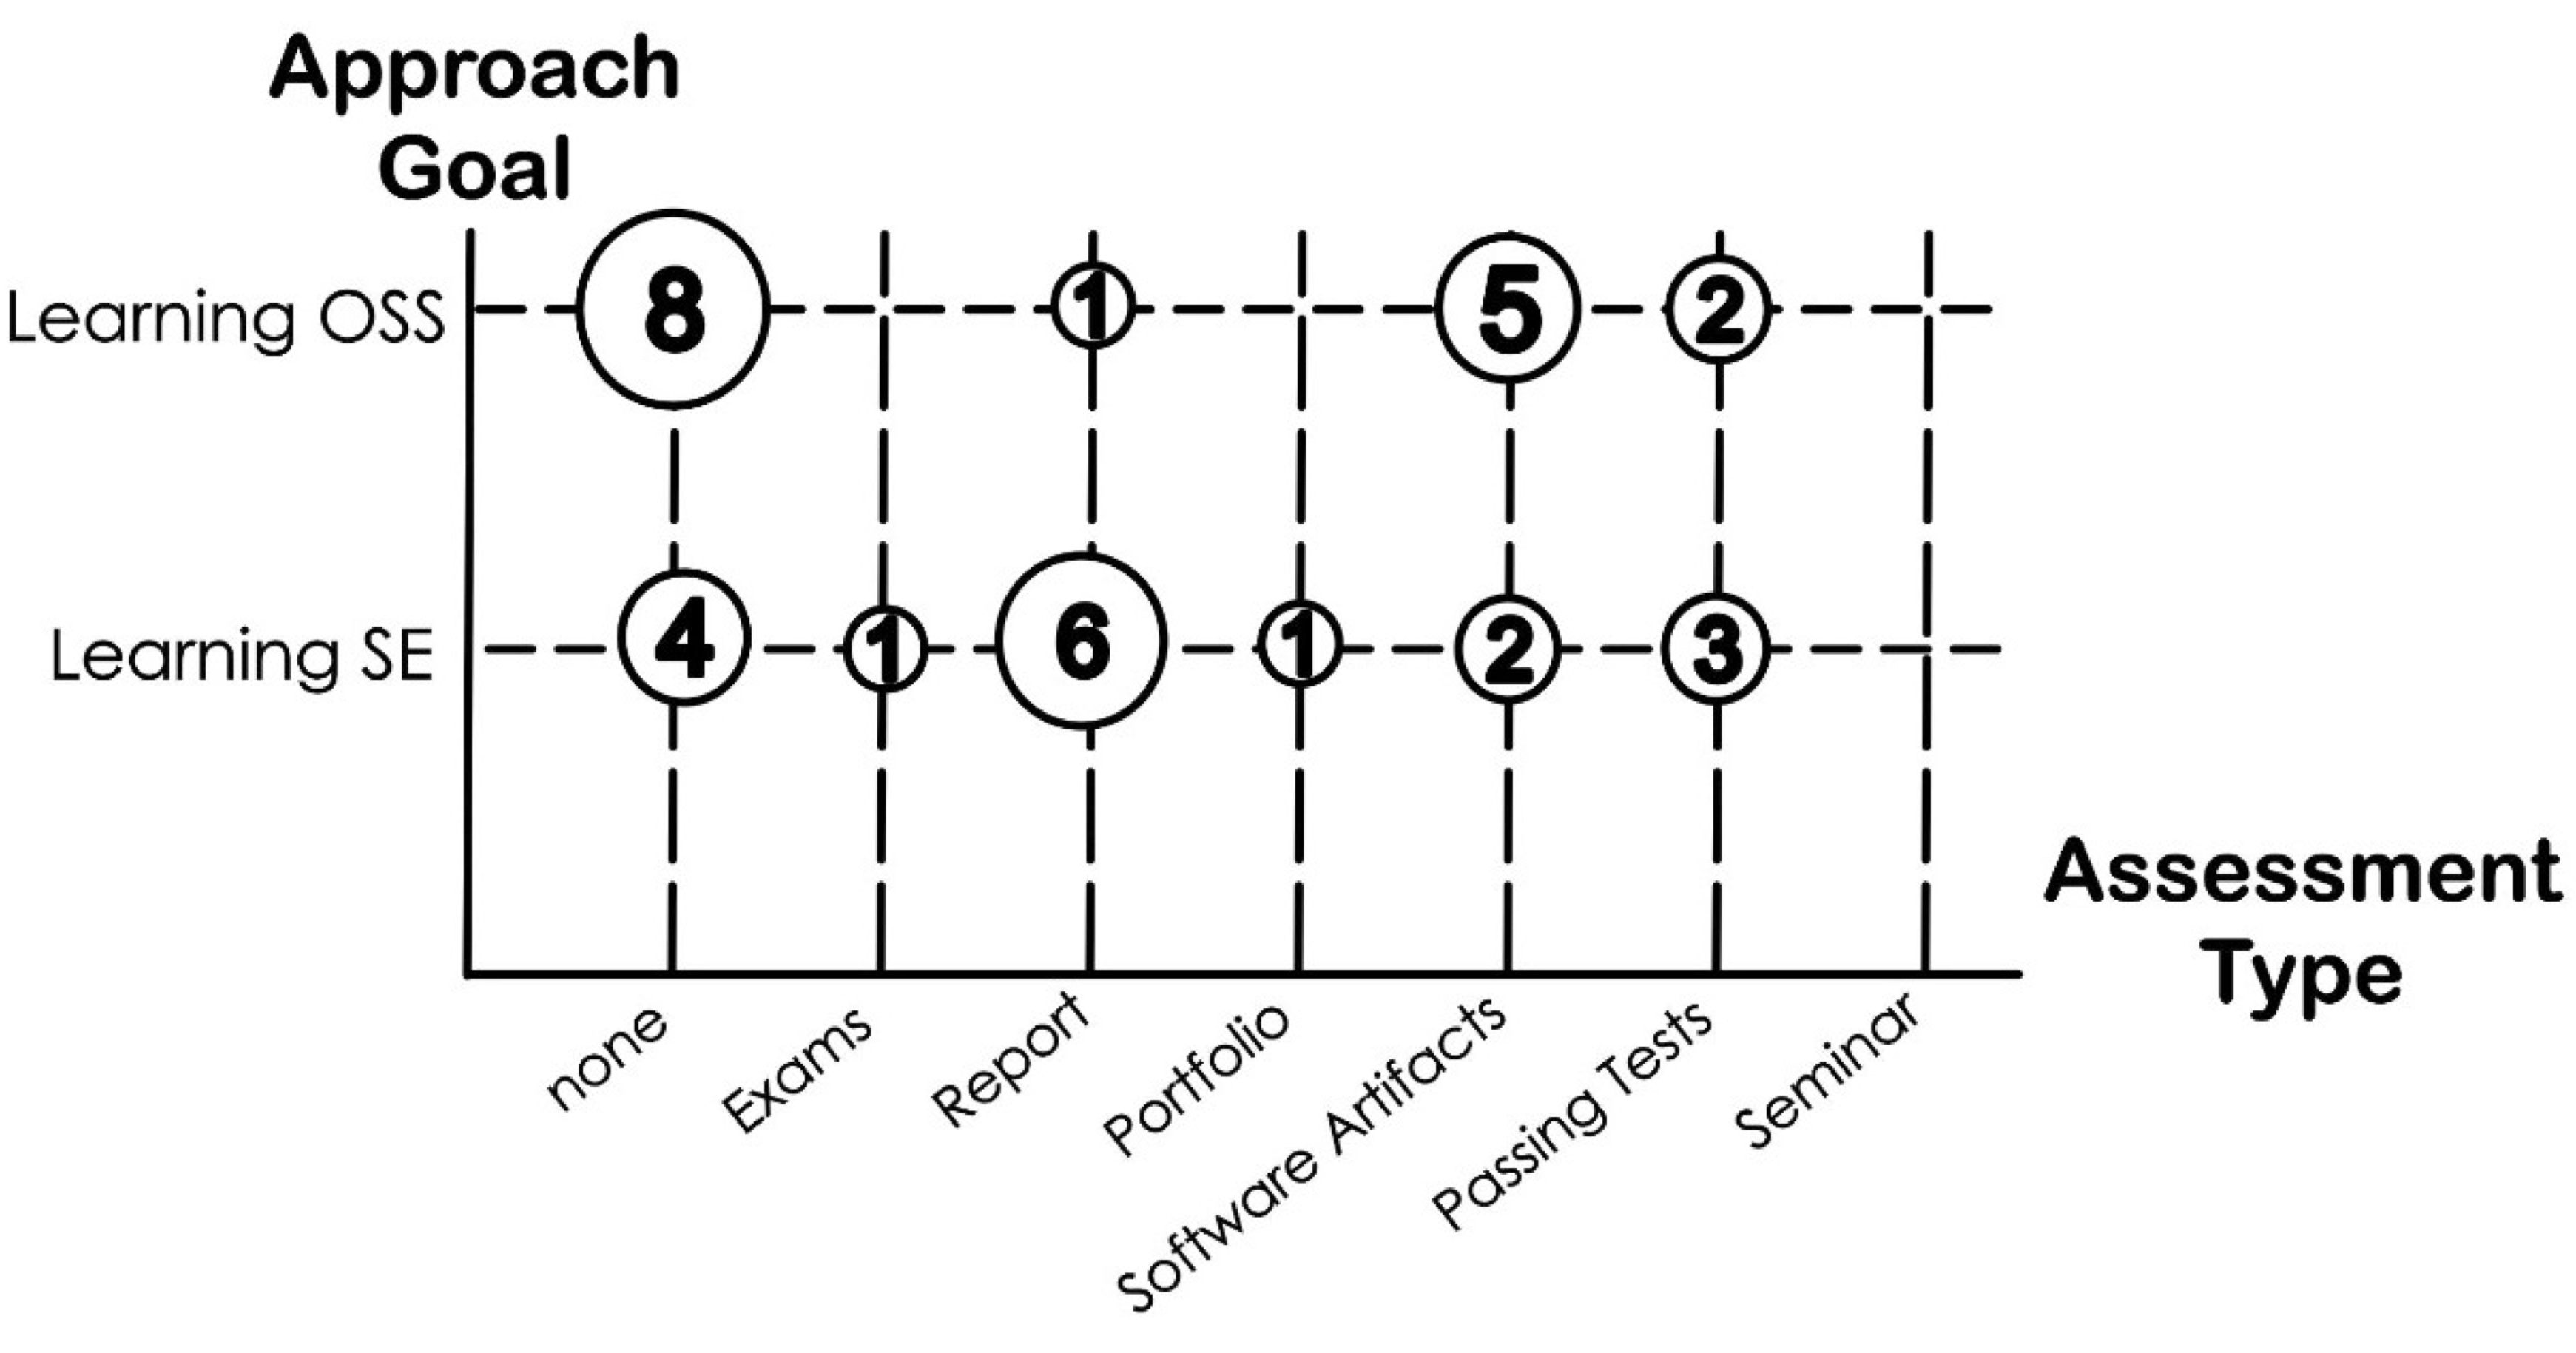
\includegraphics[width=\linewidth]{fig/mapa03.jpg}
\caption{Approach goal vs. assessment type.} \label{fig:mapa04}
\end{figure}

The map in Figure ~\ref{fig:mapa04} presents
an overview of how assessment occurs in the selected studies.
This map combines Facet 6 - Approach Goal with the Facet 5 - Assessment Type.
The primary studies are listed in Tables ~\ref{tab:approachGoalStudies} and ~\ref{tab:assessmentTypeStudies}.
% ESCLARECER: We identified the student assessment perspective from the general goals of the studies (Table ~\ref{tab:assessmentTypeStudies}).

Most studies with the general goal of teaching SE concepts and principles 
used reports (6 articles), 
passing tests (3 articles) and software artifacts (2 articles). 
The study described by \citeauthor{id4811} used exams, and the study of \citeauthor{id4811} used a portfolio. 
In studies with the goal of teaching OSS, predominantly no assessment was explicitly performed. 
From these studies, five papers used software artifacts and two other papers used passing tests. 
Only in the study of \citeauthor{id5335}, reports were used as assessment, 
although it was the predominant assessment type in the studies 
aiming to teach SE concepts and principles.

\subsection{Distribution of publications}

In the last five years, the interest of the research community
on the use of FLOSS projects in SEE has evolved. 
We present a temporal view of publications, main publication venues and the institutions that devote more effort to this subject.

\subsubsection{Temporal view}

\begin{figure}[ht]
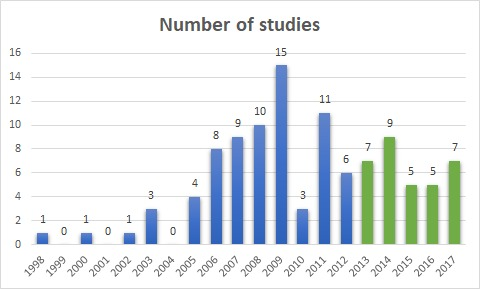
\includegraphics[width=\linewidth]{fig/number_of_studies.jpeg}
\caption{Publications vs. year.} \label{fig:publicationsvsyear}
\end{figure}

Figure~\ref{fig:publicationsvsyear} shows the distribution of publications over the years. 
The green bars refer to the number of studies identified 
in this present mapping. 
There has been a growing interest in this subject over the years. We notice an almost constant interest after a 2009 peak and a sharp fall in 2010. There is a balance in the number of studies that were published in the last five years, with a small increase in 2017 compared to 2016.

\subsubsection{Publication venues}

\begin{table}
\caption{Main Publication Venues}
{\begin{tabular}{p{3.05in}|c}
\textbf{Venue} & \textbf{\#} \\ \hline
FIE - Frontiers in Education Conference  & 3 \\
ICCSE - Intern. Conference on Computer Science \& Education & 3 \\
SIGCSE - ACM Technical Symposium on Computer Science Education & 2 \\
CSEE\&T - Conference on Software Engineering Education and Training & 2 \\
ASEE Annual Conference and Exposition & 2 \\
Journal of Computing Sciences in Colleges & 2
\end{tabular}} 
\label{tab:publicationVenue}
\end{table}


Table~\ref{tab:publicationVenue} presents the distribution of articles by venue, considering venues that published two or more selected papers. The complete set of publication venues (each with only article from the 33 selected articles) 
can  be found in our mapping study website\footnote{https://moara.github.io/mapping/}.  Most studies are still published in important conferences, 
such as the Frontiers in Education Conference (FIE) and the ACM Technical Symposium on Computer Science Education (SIGCSE). 
In the previous mapping, the Annual Conference on Innovation and Technology in Computer Science Education (ITiCSE) was identified as the second largest publication venue. In this mapping, however, only one paper was published in this conference.
The International Conference on Computer Science \& Education (ICCSE), not
identified in the previous mapping, shows up with three papers included in this update.

Figure~\ref{fig:temporalViewpublicationsources} shows how this topic has been addressed in the last five years. As in the previous systematic mapping, conferences remain the typical place to publish results (19 papers). Journals are the second most popular venue (9 papers). There was only one paper published in 2017 in both workshops and as books or book chapters. Finally, symposiums were also popular for publishing results, both in 2014 (3 paper) and in 2017 (1 paper).

\begin{figure}[ht]
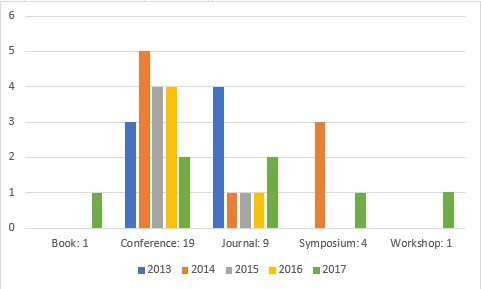
\includegraphics[width=\linewidth]{fig/types_of_venue.jpeg}
\caption{Temporal view and publication venues.} \label{fig:temporalViewpublicationsources}
\end{figure}

\subsubsection{Active research communities}

To learn which institutions have devoted effort to studying student participation in FLOSS projects as an approach to learn SE, we looked at affiliation details in our selected studies.
Table~\ref{tab:communities} summarizes the communities that had at least two selected  publications in this mapping study. 

\begin{table}[htb]
\caption{Active Research Communities}
{\begin{tabular}{p{3in}|c}
\textbf{Institutions} & \textbf{\#} \\ \hline
Drexel University, US & 7 \\
Western New England University, US & 7 \\
University of Connecticut, US & 4 \\
Nassau Community College, US & 3\\
Western Oregon University,  US & 3\\
Northern Arizona University, US & 2\\
California State University, Chico, US & 2\\
University of Minho, Portugal & 2\\
The College of New Jersey, US & 2\\
Muhlenberg College, US & 2\\
Moravian College, US & 2
\end{tabular}}
\label{tab:communities}
\end{table}



% Posicionei manualmente
\begin{figure*}[ht]
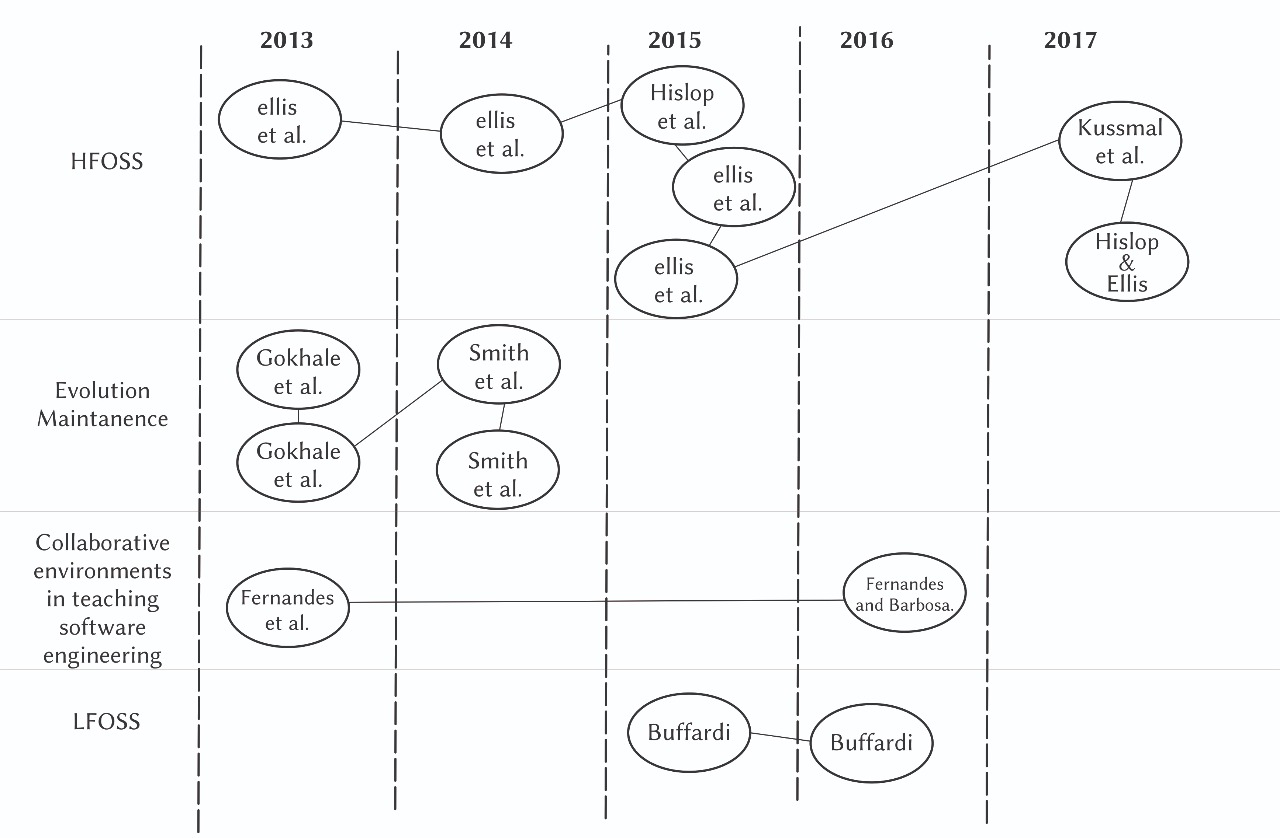
\includegraphics[width=.8\linewidth]{fig/long_term.jpeg}
\caption{Long-term projects.} \label{fig:longterms}
\end{figure*}

Communities such as Drexel University and Western New England University, 
which are related to the Humanitarian Free and Open Source Software project (HFOSS), continue to produce the largest number of studies. These communities reeived contributions from other communities that were not identified in the previous mapping. 
They are: 
Nassau Community College, Muhlenberg College, The College of New Jersey, Western Oregon University, Moravian College. 
Among the communities cited in \citeauthor{2015:CSE:nascimento} as contributors to HFOSS, only Bowdoin College was identified in our mapping. 
Drexel University and Western New England University keep very relevant 
to the research community, not only because of the number of published studies, 
but also because of their involvement with a number of other communities. 
We have not identified Trinity College community-related publication within the past five years, although they have published 12 studies in the previous mapping. 
Regarding the Aristotle University of Thessaloniki and North Carolina State University, 
who respectively published four and three papers in the previous mapping, 
we found only one study in each of them.
The University of Connecticut published two papers in 2012 
(which were previously identified), 
and four papers between 2013 and 2014. 
After that, we did not find other publications from this community 
about the use of FLOSS in SEE.

Two new communities appeared in the current mapping: 
University of Minho, which published two studies related to collaborative environments in teaching software engineering (FLOSS approach), and Northern Arizona University, which attracted attention by having two Brazilian authors 
(an Associate Professor at the Northern Arizona University (NAU) and member of the Computer Science Graduate Program at the University of São Paulo, and a Post-Doctoral Scholar at the School of Informatics, Computing and Cyber-Systems at NAU, and Assistant Professor at the Federal University of Technology - Paraná). 
They conducted research related to supporting newcomers in open source software development communities, including student involvement in FLOSS projects.

\subsection{Long-term projects}

As we read the articles included in the mapping, we tried to capture the  maturity of each solution proposal in each study, based on how long or how many times it had been applied. 
The scenario is similar to the previous mapping, with studies strongly related to others, and with few cases, since most of the identified studies continue to apply the proposed solution only once. Figure~\ref{fig:longterms} presents studies whose solution proposals were applied twice or more, and each linked set of nodes represents one identified project. 

The largest identified project was HFOSS, with seven studies.  \citeauthor{id1193} describes a workshop held to prepare faculty members to deliver courses in which students participate in HFOSS software development projects. The 2014 study \cite{id5335} and one 2015 study \cite{id4966} describe student learning within the environment of an HFOSS project. The other two 2015 studies (\cite{id5147, id17830})
report students' opinions about the learning and impact of their participation in an HFOSS project. After one year without particular publications on the use of open source projects in SEE, in 2017 we identified two publications with general information on Humanitarian Open Source Software in Computing Education \cite{id1097,id18359} and information to faculty and students on how to participate in the Humanitarian Free and Open Source software OpenFE and OpenPath.

The University of Connecticut has developed a long-term project. The first studies published in 2013 \cite{id17800,id0135} describe experiences and lessons learned from using FLOSS to teach software maintenance and evolution. 
The following papers, published in 2014 \cite{id17796,id5357},
refer to the search, by instructors and students, of projects suitable for use in SEE with a focus on maintenance and evolution.

The study of \citeauthor{id4815} is based on a pilot project in teaching and learning software engineering that has been carried out for two years. 
The first findings were reported by \citeauthor{id5546} in 2013.

In 2015, \citeauthor{id1088} described the Localized Free and Open Source Software organization - LFOSS (an
experimental approach to combine advantages of collaborating
with industry with maintaining existing open source projects), and reports initial findings from software engineering students' involvement. In this study, he also describes the Chico Open Source Consortium (COSC) as a group in Chico, California, to foster collaboration between California State University-Chico (CSU Chico) students and local software professionals in open source projects. In the following year, a new report of a more realistic software development experience was published, continuing to focus on LFOSS \cite{id4663}.
